\documentclass[12pt]{gsis}
\usepackage[misc]{ifsym}
\usepackage{graphicx,subfigure}
\usepackage{hyperref,caption}
\usepackage[para,online,flushleft]{threeparttable}
\usepackage{multirow,booktabs}
\usepackage{geometry}
\usepackage{tabularx}
\usepackage{tikz}
\usepackage{pgfplots}
\pgfplotsset{compat=1.17}
\usetikzlibrary{positioning, arrows.meta}
\usepackage{pifont}
\newcommand{\cmark}{\ding{51}}
\newcommand{\xmark}{\ding{55}}
\usepackage{natbib}% Citation support using natbib.sty
\bibpunct[, ]{(}{)}{;}{a}{}{,}% Citation support using natbib.sty

%%% Project macros
\newcommand{\sys}{GeoSemantics}
\newcommand{\patat}[1]{P@#1}

\graphicspath{{figs/}{paper_figures/}{validation_results/}{baseline_comparison/}}

\begin{document}

\copyrightyear{2026}
\datereceived{ xx xx 2026}
\dateaccepted{ xx xx 2026}

\title{GeoSemantics: An Interactive Engine for Explainable, Multi-Scale Place Character from Heterogeneous OpenStreetMap Graphs}

\author[a,b]{Angeliki Grammatikaki}
\author[a,b]{Milena Vuckovic}
\author[a]{Manuela Waldner}
\affil[a]{Institute of Visual Computing and Human-Centered Technology, TU Wien, Vienna, Austria}
\affil[b]{VRVis GmbH, Vienna, Austria}

\thanks{\textbf{CONTACT:} Angeliki Grammatikaki \quad \Letter : angiegram@icloud.com} % angeliki.grammatikaki@tuwien.ac.at

\keywords{GeoAI; graph attention networks; place embedding; OpenStreetMap; contrastive learning; explainable AI; interactive cartography}

\Abstract{Understanding the functional character of a place (e.g., what distinguishes a historic market square from a residential suburb, or a mountain trailhead from a logistics zone) remains a core challenge in urban analytics, traditionally requiring proprietary, visual, or manually labeled data. We present a self-supervised system that learns interpretable place character representations exclusively from OpenStreetMap data. Our heterogeneous, multi-scale graph attention network (Typed-GAT) models each location as a spatial graph at radii of 200m, 700m, and 2km, distinguishing features like points of interest and transportation infrastructure. Trained by InfoNCE-based contrastive learning, it generates compact location embeddings and easily readable character fingerprints. A benchmark of 400 expert-analyzed locations in Austria, representing 10 different types, reveals that Typed-GAT improves on the separability of embeddings and Silhouette Scores relative to the base model, Flat-GAT. Although Urban2Vec and Tile2Vec, which rely on street-level and satellite imagery, achieve stronger nearest-neighbor retrieval, Typed-GAT offers a better global embedding architecture. This enables better semantic clustering, continuous character mapping, and clearer visual analytics. The models are components of an interactive engine that makes predictions understandable, demonstrates attention visualization, and enables fast ``what-if'' scenarios in under one second.}

\newgeometry{top=20.0mm,bottom=40.0mm,left=15mm,right=15mm,headsep=8mm}
\maketitle
\restoregeometry
\newpage


\section{Introduction}

Place character --- the qualitative sense of what a location is, beyond zoning code \citep{tuan1977space} --- shapes critical decisions in urban planning, retail siting \citep{Montgomery01021998}, and everyday human wayfinding in complex landscapes \citep{lynch1960image}. 
While humans intuitively grasp the character of a place (e.g., instantly distinguishing a bustling, historic market square from a quiet residential suburb), computational systems, given only a geographic coordinate or a postal code, remain blind to this functional reality. This gap is particularly important in frequently neglected rural, alpine, and peri-urban areas. In these locations, the OSM data signal is weaker --- fewer tagged features, lower tagging density --- yet the functional differences between a trailhead and a logistics zone are just as pronounced as those between two city blocks.

To bridge this gap, modern computational systems model place character using auxiliary sources such as mobility traces~\citep{place2vec}, street-level imagery~\citep{urban2vec}, or satellite imagery \citep{tile2vec}. However, these sources are proprietary, privacy-sensitive, and unevenly distributed, failing outside instrumented city cores \citep{Fonte-2017}. Mobility traces and check-in logs \citep{cheng2011exploring} are proprietary, privacy-sensitive, and sparse outside metropolitan cores, meaning they fail in rural, peri-urban, or developing areas. Street-level and satellite imagery capture visual style rather than functional character (e.g., confusing a public café with a private office within identical buildings)~\citep{10.1145/2830541}, whilst incurring significant acquisition and processing costs. Manual annotations also age quickly and struggle to transfer across cultural regions.

OpenStreetMap (OSM) provides a compelling alternative \citep{10.1109/MPRV.2008.80}. It is global, free, community-updated \citep{goodchild2007citizens}, and already encodes a rich, structured vocabulary of POIs, transport infrastructure, and natural features. The open research question is whether this topological vocabulary, structured as a spatial graph, is sufficient to learn a representation of place character without auxiliary data or labels, and whether that representation can be made legible to a human user rather than remaining an opaque vector.

We present GeoSemantics, a self-supervised spatial engine that constructs multi-scale local graphs from raw OSM features around any coordinate and encodes them via a multi-scale Graph Attention Network (Typed-GAT) based on the GATv2 architecture \citep{brody2022attentivegraphattentionnetworks}. Trained purely via contrastive learning \citep{DBLP:journals/corr/abs-1807-03748}, the system produces dense 64-dimensional location embeddings for similarity retrieval and 7-dimensional interpretable character fingerprints derived by a decoupled saliency network, served through a real-time web application.

Our primary contributions are:
\begin{enumerate}
\item {Heterogeneous multi-scale graph construction}: We extend a GATv2 backbone \citep{brody2022attentivegraphattentionnetworks} with a five-class node-typing scheme (POI, Transport, Natural, Built, Place) and bearing-aware edge encodings across three spatial scales (200m, 700m, 2km), enabling the GNN to distinguish map elements and their spatial relationships at block, neighborhood, and district level.
\item {Self-supervised training with decoupled saliency readout}: We train the GNN via InfoNCE contrastive learning under node-masking, requiring no labels. A lightweight saliency network decodes location embeddings into a 7-dimensional character fingerprint. The fingerprint's interpretability is deliberately decoupled so that the readout layer can be updated independently of the GNN.
\item {Interpretable, interactive reasoning engine}: The models are served through a real-time application that exposes reasoning at three levels: natural-language explanations; saliency-thresholded attention overlays and precomputed map layers; and a counterfactual sandbox that reruns inference on user-modified graphs in under a second.
\end{enumerate}

The practical motivation for this interactive framing is worth stating directly. A practitioner presented with a label — say, ``Tourist Destination'' for a candidate development site — needs to trace that label back to the specific POI composition that produced it, verify which spatial scale is most influential, and test whether a proposed hotel cluster or the removal of an existing parking facility would shift the reading. Static thematic maps and offline embedding files cannot support this workflow: they fix the prediction at the time of computation and provide no mechanism for local intervention or scale-level interrogation. GeoSemantics is designed to close this loop by exposing every computational step --- from raw OSM tag ingestion, through graph construction and GNN message passing, to fingerprint rendering and archetype matching --- as an interactive, sub-second query accessible through a standard web browser. The system is therefore simultaneously a research contribution in spatial representation learning and a practical tool for exploratory place reasoning.

The remainder of this paper is organized as follows. Section~\ref{sec:related} surveys related work in place representation, heterogeneous graph learning, explainability, and interactive visual analytics. Section~\ref{sec:method} details the data pipeline, model architecture, training procedure, and interactive engine. Section~\ref{sec:eval} presents quantitative benchmark results, per-class analysis, ablation experiments, and case studies in temporal drift and counterfactual simulation. Section~\ref{sec:discussion} discusses performance trade-offs, failure modes, and open directions, and Section~\ref{sec:conclusion} concludes.

\section{Related Work} \label{sec:related}

\textbf{Place Representation and Urban Embeddings}
Place2Vec~\citep{place2vec} learns POI co-occurrence embeddings from check-ins, capturing behavior-driven signals but failing beyond wealthy, instrumented urban cores. This sits within a broader family of region-embedding methods --- including POI2Vec~\citep{3298239.3298256} and Region2Vec-style approaches~\citep{luo2022urbanregionprofilingmultigraph} --- that similarly depend on mobility or check-in density and inherit the same coverage bias. Image-based techniques include Urban2Vec~\citep{urban2vec} and Tile2Vec~\citep{tile2vec}, which use street- or satellite-level imagery and carry corresponding acquisition costs. Structure-only techniques operate over road networks or POI proximity graphs: space syntax~\citep{hillier1984social} computes salience from street-network structure, while DeepWalk~\citep{Perozzi_2014} and Node2Vec~\citep{grover2016node2vecscalablefeaturelearning} apply random-walk skip-gram models to homogeneous proximity graphs but cannot distinguish edge semantics (e.g. road-to-caf\'e vs.\ caf\'e-to-caf\'e) --- a limitation our typed-edge design directly addresses. A recent survey of location encoding for GeoAI~\citep{mai2022review} identifies the lack of structural, topology-aware representations as a key gap in the literature, positioning graph-based spatial encoders as a promising direction for bridging raw geographic coordinates and functional place semantics.

Feature salience connects our work to landmark models that incorporate visual, semantic, and structural aspects~\citep{Caduff, 10.1007/3-540-45799-2_17}, which we approximate by weighting OSM features using distance centrality, category uniqueness, and degree. Landmark salience has been studied extensively in urban settings dominated by buildings, but rarely in rural or alpine contexts --- precisely where our heterogeneous graph shows its largest gains. This asymmetry mirrors a broader pattern in the volunteered geographic information (VGI) literature: OSM's coverage and tagging density are known to be uneven and community-driven~\citep{haklay2010good, goodchild2007citizens, Fonte-2017}, a limitation our node-masking augmentation is designed to tolerate rather than assume away.

\textbf{Heterogeneous and Self-Supervised Graph Learning}
Heterogeneous GNNs that separate node and edge types --- HAN~\citep{wang2021heterogeneousgraphattentionnetwork}, HGT~\citep{hu2020heterogeneousgraphtransformer}, RGCN~\citep{schlichtkrull2017modelingrelationaldatagraph}, and HetGNN~\citep{10.1145/3292500.3330961} --- were developed primarily for knowledge graphs and citation networks. Applying this family to geospatial data introduces distinct constraints: the type taxonomy must fit the OSM tagging schema rather than a curated ontology, edges must encode continuous spatial relations (bearings, distances) alongside discrete types, and pooling must handle extreme class imbalance (Transport nodes constitute $\approx$40\% of our corpus). Our GATv2 backbone~\citep{brody2022attentivegraphattentionnetworks} adapts to these constraints via per-type embedding tables, type tokens, and stratified gated pooling.

On the training side, self-supervised graph representation learning has converged on contrastive objectives such as SimCLR-style instance discrimination~\citep{DBLP:journals/corr/abs-2002-05709}, Deep Graph Infomax~\citep{velicković2018deepgraphinfomax}, and masked-node reconstruction as in GraphMAE~\citep{hou2022graphmaeselfsupervisedmaskedgraph}. We adopt node-masking as our augmentation for a domain-specific reason: POI omission is a routine data-quality event in OSM, so training for invariance to it directly targets the sparsity regime documented in the VGI literature above, rather than treating masking as a generic regularizer.

\textbf{Explainability for Graph Neural Networks}
A separate line of work asks how to make GNN predictions legible rather than just accurate. GNNExplainer~\citep{ying2019gnnexplainergeneratingexplanationsgraph} and related post-hoc attribution methods~\citep{kakkad2023surveyexplainabilitygraphneural} identify influential subgraphs after training, while raw attention weights have been criticized as an unreliable explanation signal on their own~\citep{jain2019attentionexplanation, serrano2019attentioninterpretable}. Our interactive engine sidesteps this critique architecturally: saliency is produced by a dedicated, decoupled network trained against an interpretable formula, rather than read directly off GATv2's attention weights, which we use only as a supplementary visual overlay rather than the primary explanation mechanism. The decoupling means the readout layer can be updated --- e.g., to incorporate user corrections or newly defined landmark taxonomies --- without retraining the GNN backbone.

\textbf{Interactive Visual Analytics for Urban Spatial Data}
Translating latent spatial representations into practitioner-facing tools requires interactive reasoning environments in which users can interrogate, manipulate, and compare model outputs in real time. Functional region inference approaches~\citep{10.1145/2339530.2339561, luo2022urbanregionprofilingmultigraph} characterize neighborhoods from mobility and POI data alone, but their outputs are typically static thematic maps or pre-computed cluster labels, offering no mechanism to query \emph{why} a region received a particular classification or to test the effect of a proposed urban intervention. Visual analytics systems for geospatial machine learning~\citep{Andrienko2021} have explored linked-view architectures that combine geographic maps with embedding projections, but almost exclusively in a read-only mode: the user can inspect the model but not modify its inputs. The closest work in spirit to ours is ``What-if'' prototyping for urban design~\citep{Miao2018}, where parametric models allow users to adjust land-use variables and see projected outcomes. HomeFinder~\citep{10.1145/3173574.3173821} pursues a related goal for residential location search, letting users specify opportunity criteria (proximity to schools, parks, transport) and instantly re-rank neighborhoods via a linked map and ranking view. GeoSemantics extends both paradigms into the learned-embedding space: what-if edits are applied directly to the OSM graph, and the full GNN inference pipeline re-executes on the modified graph, producing an updated embedding and fingerprint rather than a rule-based proxy --- making the counterfactual grounded in the same representation used for similarity retrieval and archetype matching.

Landmark-based cognitive mapping~\citep{lynch1960image, Caduff, 10.1007/3-540-45799-2_17} links individual map features to place identity and navigational legibility, but these models operate at the conceptual level and have not been integrated into live, editable inference pipelines backed by learned representations. Dimensionality-reduction projections such as UMAP~\citep{mcinnes2020umapuniformmanifoldapproximation} --- part of a broader family of high-dimensional visualization techniques surveyed in~\citet{liu2017visual} --- are widely used in spatial representation learning to visualize embedding quality, but are typically rendered as static scatterplots decoupled from their geographic source data. GeoSemantics connects these threads into a single interactive system in which the UMAP landscape and the geographic basemap are linked bidirectionally: navigating either view updates the other in real time, allowing a user to observe where a location falls in embedding space while simultaneously seeing its geographic context. To our knowledge, this is the first graph-level what-if interface for place character that supports sub-second re-inference on live OSM data.

\section{Methodology}
\label{sec:method}

GeoSemantics constructs typed, multi-scale spatial graphs from raw OSM features around any user-defined geographic coordinate, processes these structured representations using a multi-scale graph attention network, and exposes the resulting embeddings and explainable character fingerprints through an interactive, web-based reasoning engine.

\subsection{Data and Feature Encoding}
\label{sec:data}

The dataset is a static extract of Austrian OSM point features from the Geofabrik national dump~\citep{geofabrik2024}, consisting of $\mathbf{2{,}453{,}475}$ nodes after geometry simplification to points. Each node in our extract carries up to four dedicated semantic columns (\texttt{highway}, \texttt{natural}, \texttt{place}, \texttt{man\_made}) alongside an \texttt{other\_tags} field holding all remaining key--value pairs. A primary category is derived from the first non-empty dedicated column; the \texttt{other\_tags} field is then parsed for amenity, shop, tourism, and historic keys as a secondary pass. This yields 222 distinct primary categories across the full corpus. Each node also receives a 32-dimensional bag-of-keys feature vector, where each dimension indicates the presence or absence of a particular tag key in \texttt{other\_tags}. Tag values are excluded to prevent the model from overfitting to named entities.

All nodes have been tagged as belonging to one of the five semantic categories, determined by applying a deterministic rule in the following priority sequence: POI $>$ Transport $>$ Natural $>$ Built $>$ Place. The use of the priority sequence is necessary because it eliminates potential confusion when a node contains attributes from more than one semantic category. Semantic categories correspond to different sets of OSM keys as shown in Table~\ref{tab:nodetypes}. Transport nodes account for most nodes (approximately 40\%), since all highway segments produce them, along with railways and public transport points.

\begin{table}[htbp]
\centering
\begin{tabularx}{\textwidth}{lXr}
\toprule
\textbf{Type} & \textbf{OSM signal} & \textbf{Approx.\ \%} \\
\midrule
POI (0)       & amenity, shop, tourism, leisure, historic, healthcare & 12 \\
Transport (1) & \texttt{highway} column; railway, public\_transport & 40 \\
Natural (2)   & \texttt{natural} column; waterway, natural landuse & 8 \\
Built (3)     & building, man\_made, power, built landuse & 25 \\
Place (4)     & \texttt{place} column; remaining landuse, barrier & 15 \\
\bottomrule
\end{tabularx}
\caption{Node type classification scheme. Priority order prevents ambiguity.}
\label{tab:nodetypes}
\end{table}

Each node carries a 37-dimensional initial embedding: a 32-dimensional bag-of-keys feature vector, a one-hot node-type indicator (5 dimensions). The bag-of-keys vector records the presence or absence of 32 high-frequency OSM tag keys selected by term frequency across the Austrian corpus, with each key capped at two occurrences per document to prevent individual tags from dominating the vocabulary. Tag \emph{values} are deliberately excluded to prevent the model from memorizing named entities (e.g., a café called ``Kaffehaus Wien'') rather than learning structural category relationships that generalize across locations.

The seven-dimensional character fingerprint produced at inference spans seven interpretable semantic dimensions: Urban/Commercial, Tourism, Heritage, Nature, Transport, Built/Infra, and Community. Each OSM node is deterministically mapped to one dimension by a secondary tag-key lookup applied after primary node-type assignment. Table~\ref{tab:fingerprint} specifies the complete mapping. Tourism nodes carry \texttt{tourism=*} tags; Heritage nodes \texttt{historic=*}; Nature nodes \texttt{natural=*} or \texttt{landuse=forest/meadow}; Transport nodes \texttt{highway=*} or \texttt{railway=*}; Built/Infra nodes \texttt{building=*}, \texttt{man\_made=*}, \texttt{power=*}, or \texttt{landuse=industrial/residential}; Community nodes \texttt{leisure=*}, \texttt{healthcare=*}, \texttt{sport=*}, or \texttt{place=*}; and all remaining POI nodes default to Urban/Commercial. Critically, nodes tagged as \texttt{amenity=cafe} or \texttt{shop=souvenir} contribute to Urban/Commercial rather than Tourism because OSM's tag vocabulary reserves the \texttt{tourism=*} key for named attractions and accommodation: the surrounding commercial fabric of any tourist district is therefore systematically miscategorized in a raw tag-count model. This mapping is transparent and deterministic, allowing the natural-language generator to report not only the dominant character label but also which specific named POIs drove each fingerprint dimension.

\begin{table}[htbp]
\centering
\begin{tabularx}{\textwidth}{lX}
\toprule
\textbf{Fingerprint dimension} & \textbf{Primary OSM keys} \\
\midrule
Urban/Commercial & \texttt{amenity}, \texttt{shop}, \texttt{office}, \texttt{craft}, \texttt{club}, \texttt{gambling}, \texttt{landuse=commercial/retail} \\
Tourism          & \texttt{tourism=hotel/attraction/museum/gallery/viewpoint} \\
Heritage         & \texttt{historic=*}, \texttt{tourism=museum/gallery} \\
Nature           & \texttt{natural=*}, \texttt{waterway=*}, \texttt{landuse=forest/meadow/heath} \\
Transport        & \texttt{highway=*}, \texttt{railway=*}, \texttt{public\_transport=*}, \texttt{aeroway=*} \\
Built/Infra      & \texttt{building=*}, \texttt{man\_made=*}, \texttt{power=*}, \texttt{landuse=industrial/residential} \\
Community        & \texttt{leisure=*}, \texttt{healthcare=*}, \texttt{sport=*}, \texttt{place=*} \\
\bottomrule
\end{tabularx}
\caption{Deterministic OSM-tag-to-fingerprint-dimension mapping. Each node receives exactly one dimension via this lookup applied after node-type assignment.}
\label{tab:fingerprint}
\end{table}

The 7,627 locations for which fingerprints are precomputed at application start-up were drawn by spatially stratified sampling across Austria's nine federal states, oversampling alpine districts (Tyrol, Salzburg, Carinthia) to ensure coverage of sparse Rural and Alpine archetypes that are underrepresented in population-density-proportional sampling. Specifically, each federal state was allocated a quota of locations proportional to its land area rather than its population, which increases the share of alpine and rural locations by approximately 3$\times$ relative to a population-weighted draw. Each candidate location was required to have at least one OSM node within 200m and five within 2km; this threshold filters out water bodies, uninhabited alpine ridge-lines, and border regions with insufficient tag density for meaningful graph construction, while retaining mountain valley settlements and alpine resort villages that constitute an important part of Austria's place-character diversity. Candidate locations that failed this threshold were replaced by a neighboring point shifted 500m in a random direction until the criterion was satisfied or a maximum of ten retries was exceeded, in which case the location was dropped from the precomputed set entirely. The resulting coverage is approximately one precomputed location per 11km$^2$ of Austrian territory, concentrated in populated valleys and urban centers but with non-trivial coverage of alpine national parks and rural lowlands.

For any user-queried coordinate, three directed $k$-NN scale graphs ($k=8$) are built at 200m (block), 700m (neighborhood), and 2km (district) to capture multi-scale context. Edges encode geodetic distance expanded into sinusoidal harmonics~\citep{vaswani2023attentionneed} and bearing decomposition $(\sin\theta_{ij}, \cos\theta_{ij})$, making the graph network orientation-aware: a caf\'{e} adjacent to a road to its north receives different attention weights than the same caf\'{e} adjacent to a road to its west. A binary flag indicating whether source and target share the same primary category completes the edge feature vector, helping the model capture local category homophily.

\subsection{Model Architecture and Training}
\label{sec:architecture}

We compare a Flat-GAT baseline with a Typed-GAT extension. Both generate 64-dimensional embeddings and 3-dimensional scale-attention weights.

\textbf{Flat-GAT} processes all nodes uniformly. Category embeddings are combined with coordinates, and each scale is processed via two GATv2 layers~\citep{brody2022attentivegraphattentionnetworks} with learnable scale tokens, using gated mean pooling and cross-scale attention.

\textbf{Typed-GAT} uses independent category embedding tables for the five node types, learnable segment-type tokens $\mathbf{T} \in \mathbb{R}^{5 \times 64}$ --- one row per node type --- analogous to segment-type tokens in BERT, which conditions the graph attention mechanism on node type. For pooling, global mean pooling is replaced by per-type gated aggregation:
\begin{equation}
\mathbf{p}_t = \frac{\sum_{i:\tau_i=t} \sigma(\mathbf{W}_g \mathbf{x}_i) \odot \mathbf{x}_i}{\sum_{i:\tau_i=t} \sigma(\mathbf{W}_g \mathbf{x}_i)}, \quad t \in \{0,\ldots,4\},
\label{eq:typepool}
\end{equation}
fused through an MLP-driven weighted sum:
\begin{equation}
\mathbf{w} = \mathrm{Softmax}(\mathrm{MLP}([\mathbf{p}_0 \Vert \cdots \Vert \mathbf{p}_4])), \quad \mathbf{h} = \sum_{t=0}^{4} w_t \mathbf{p}_t.
\label{eq:weightedpool}
\end{equation}
This prevents Transport nodes ($\approx$40\%) from drowning out sparse Natural nodes ($\approx$8\%). Trainable parameters total $\approx$43{,}500.

At each message-passing layer $\ell$, the GATv2 attention score between node $i$ and neighbor $j$ is:
\begin{equation}
e_{ij}^{(\ell)} = \mathbf{a}^{(\ell)\top} \mathrm{LeakyReLU}\!\left(\mathbf{W}^{(\ell)}\!\left[\mathbf{x}_i^{(\ell)} \Vert \mathbf{x}_j^{(\ell)} \Vert \mathbf{e}_{ij}\right]\right),
\label{eq:gatv2attn}
\end{equation}
where $\mathbf{a}^{(\ell)}$ and $\mathbf{W}^{(\ell)}$ are layer-specific learnable parameters and $\mathbf{e}_{ij}$ is the edge feature vector. Softmax-normalized weights $\alpha_{ij} = \mathrm{softmax}_{j \in \mathcal{N}(i)}(e_{ij}^{(\ell)})$ produce the updated node representation:
\begin{equation}
\mathbf{x}_i^{(\ell+1)} = \sigma\!\left(\sum_{j \in \mathcal{N}(i)} \alpha_{ij}\, \mathbf{W}'^{(\ell)}\mathbf{x}_j^{(\ell)}\right).
\label{eq:gatv2update}
\end{equation}
The critical advantage of GATv2 over its predecessor is that $\mathbf{W}^{(\ell)}$ is applied before concatenation, enabling the attention function to condition jointly on source and target features simultaneously~\citep{brody2022attentivegraphattentionnetworks}. In the geospatial context this matters: the relevance of a Transport node to a Heritage node in a historic quarter depends on their spatial relationship in a way that is not captured by querying each independently. In Typed-GAT, the node feature $\mathbf{x}_i^{(\ell)}$ is augmented with the type-segment token $\mathbf{T}[\tau_i]$ before Eq.~\eqref{eq:gatv2attn}, conditioning attention on node type from the first layer onward. The edge feature $\mathbf{e}_{ij}$ concatenates: sinusoidal distance harmonics (8 dimensions), bearing decomposition $(\sin\theta_{ij}, \cos\theta_{ij})$ (2 dimensions), and a homophily flag (1 dimension), for an 11-dimensional edge representation.

\textbf{Training} We optimize NT-Xent contrastive loss over positive pairs created by masking node categories and features with $p=0.20$:
\begin{equation}
\mathcal{L} = \frac{1}{2}\!\left[ \mathcal{H}(\mathbf{z}_1 \mathbf{z}_2^\top / \tau,\,\mathbf{I}) + \mathcal{H}(\mathbf{z}_2 \mathbf{z}_1^\top / \tau,\,\mathbf{I}) \right],
\label{eq:infonce}
\end{equation}
with temperature $\tau=0.07$. The NT-Xent objective maximizes agreement between two augmented views of the same location (positive pairs) while pushing apart views of different locations (negatives) within the same batch. With batch size 32 there are $32 \times 31 = 992$ negative pairs per step, providing sufficient contrastive signal without the memory overhead of a dedicated momentum queue. The temperature $\tau=0.07$ was selected to concentrate gradients on hard negatives --- pairs of locations that are genuinely spatially distinct but have similar OSM tag distributions (e.g., two urban centers in different federal states) --- following the analysis in~\citep{DBLP:journals/corr/abs-2002-05709}. Typed-GAT is trained on $N=500$ locations (batch size 32) using the Adam optimizer with a learning rate of $10^{-3}$ and a weight decay of $10^{-4}$ for up to 150 epochs. Flat-GAT is trained under the same procedure with $N=1{,}000$ locations; training sizes were selected to equalize GPU memory consumption, as Typed-GAT's five parallel type-gated aggregators consume approximately twice the per-sample memory of Flat-GAT's homogeneous pooling, making $N=500$ the practical upper bound for Typed-GAT under the same hardware budget. We apply a self-supervised masked graph autoencoder framework adapted from prior work~\citep{hou2022graphmaeselfsupervisedmaskedgraph}. For each of the $N$ training locations, two augmented views of the local heterogeneous spatial graph are generated by randomly masking each node with probability $p=0.20$. Masked nodes have their categories replaced by a special mask token and their features zeroed, forcing the model to reconstruct local place character from the surrounding topological context. This type of mask is based on incomplete OSM tagging and the absence of POIs, thereby making the representation more robust in data-scarce settings, such as rural areas and historical periods. Two masks of the same place are taken as positive samples, whereas other places in the same training sample constitute negative samples. Early stopping occurs after 15 epochs in the absence of a decrease in validation loss.

\textbf{Saliency readouts} A decoupled, two-layer GCN GNN approximates a heuristic salience formula (50\% distance centrality, 30\% category uniqueness, 20\% node degree). Saliency scores are used to construct a seven-dimensional character fingerprint by accumulating saliency-weighted category counts:
\begin{equation}
\mathbf{c}[d] = \frac{\sum_{i:\mathrm{dim}(c_i)=d} w_i}{\sum_i w_i}, \quad w_i = 0.7\,\tilde{s}_i + 0.3,
\label{eq:fingerprint}
\end{equation}
where $\tilde{s}_i$ is the normalized GCN saliency score. The fingerprint is L1-normalized and fed to a rule-based natural-language generator. The floor weight of 0.3 ensures that even low-salience nodes contribute, preventing a single dominant node from monopolizing the reading of a neighborhood.

\begin{figure}[htbp]
\centering
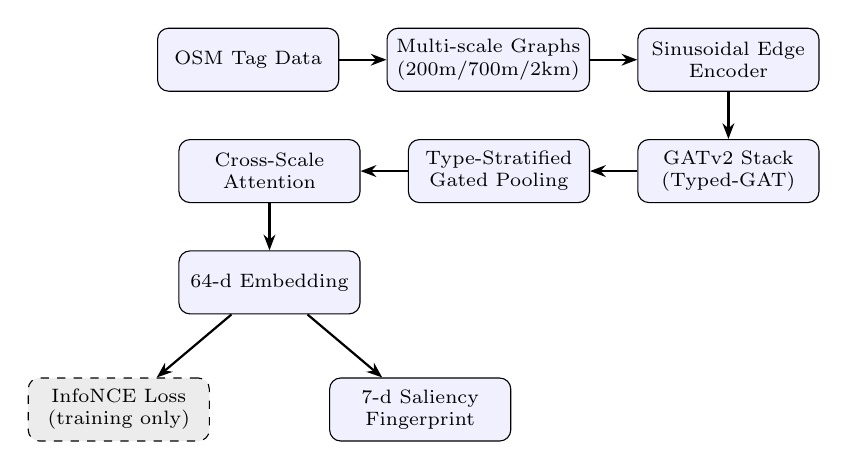
\begin{tikzpicture}[
  node distance=6mm,
  box/.style={draw, rounded corners, minimum width=2.3cm,
              minimum height=0.8cm, align=center, fill=blue!6, font=\scriptsize},
  lossbox/.style={draw, rounded corners, minimum width=2.3cm, dashed,
              minimum height=0.8cm, align=center, fill=gray!15, font=\scriptsize},
  arr/.style={-{Stealth[length=2mm]}, thick}
 ]
\node[box] (osm)  {OSM Tag Data};
\node[box, right=of osm]  (graph) {Multi-scale Graphs\\(200m/700m/2km)};
\node[box, right=of graph] (edge)  {Sinusoidal Edge\\Encoder};
\node[box, below=of edge]  (gat)   {GATv2 Stack\\(Typed-GAT)};
\node[box, left=of gat]    (pool)  {Type-Stratified\\Gated Pooling};
\node[box, left=of pool]   (cross) {Cross-Scale\\Attention};
\node[box, below=of cross] (emb)   {64-d Embedding};
\node[lossbox, below left=8mm and -4mm of emb]  (info)  {InfoNCE Loss\\(training only)};
\node[box, below right=8mm and -4mm of emb]  (char)  {7-d Saliency\\Fingerprint};
\draw[arr] (osm) -- (graph);
\draw[arr] (graph) -- (edge);
\draw[arr] (edge) -- (gat);
\draw[arr] (gat) -- (pool);
\draw[arr] (pool) -- (cross);
\draw[arr] (cross) -- (emb);
\draw[arr] (emb) -- (info);
\draw[arr] (emb) -- (char);
\end{tikzpicture}
\caption{End-to-end pipeline. The 64-d embedding feeds into an InfoNCE contrastive loss during training only (dashed, gray), and a saliency network produces the 7-dimensional interpretable fingerprint at inference.}
\label{fig:architecture}
\end{figure}

\subsection{Interactive Engine}
\label{sec:system}

The trained models are served through a web application backed by a precomputed spatial index of 2.4 million OSM nodes stored in a KD-tree for $O(\log n)$ radius queries. The end-to-end inference pipeline --- graph construction, GNN forward pass, saliency computation, and fingerprint rendering --- runs on commodity CPU hardware with a median latency of 180ms per location on a single-core query, enabling sub-second interactivity without dedicated GPU infrastructure. The application is organized around three interpretability layers and three additional interaction modes.

\emph{Point Lens (Figure~\ref{fig:lens})} is the primary entry point. Clicking any coordinate triggers a radius query across all three scale bands (200m, 700m, 2km), constructs the typed spatial graph, runs a GNN forward pass, and displays: (i) a seven-dimensional character fingerprint rendered as a color-coded proportional bar chart; (ii) three-dimensional scale-attention weights indicating which spatial scale is dominant; and (iii) a natural-language reading that names the character label, the dominant and secondary fingerprint dimensions, the three highest-saliency POIs by name, and a nearest-archetype comparison at cosine similarity. A confidence caveat is appended if OSM coverage is sparse (fewer than 20 nodes within 2km). A representative reading for Hallstatt (47.5608\textdegree{}N, 13.6477\textdegree{}E) is: \emph{``Tourist Destination, predominantly Urban (53\%) with a secondary Tourism presence (35\%). Anchored by Hallstatt Lahn (B\"ackerei), Bella Milano, and Hallstatt Damsgasse. Identity is set at the Macro (2km) scale (46\%). Closest comparable archetype: Innsbruck (76\% similarity), 94\% confidence based on 258 features.''} The multi-select POI filter allows users to suppress or highlight individual nodes and observe their marginal contribution to the fingerprint.

\emph{Attention Overlay (Figure~\ref{fig:attn})} visualizes GATv2 attention weights from the second message-passing layer as directed polylines linking POI pairs on the map. Edge color encodes source node type (Transport: blue; POI: green; Natural: teal; Built: grey; Place: purple) and edge thickness scales linearly with normalized attention weight. Only edges whose both endpoints exceed a saliency threshold of $0.3$ are rendered; self-loop attention is omitted. Comparing Flat-GAT and Typed-GAT overlays at the same location reveals a qualitative difference: Flat-GAT generates no qualifying edges in sparse alpine areas because homogeneous pooling fails to assign sufficient attention mass to rare node-type combinations, while Typed-GAT surfaces type-conditioned connections between Natural and POI nodes --- illustrating why the heterogeneous model extracts discriminative signal where the homogeneous one does not.

\emph{Continuous Semantic Layer (Figure~\ref{fig:charlayer})} renders a full-country semantic surface by interpolating a precomputed $100\times100$ grid of fingerprints (3,729 cells across the Austrian land area) using inverse-distance weighting~\citep{10.1145/800186.810616} ($k=25$, power $1.6$). The raster is rendered as an RGBA heatmap with Gaussian blur ($\sigma=8$px) and exponential color mixing to suppress speckle. The layer resamples only viewport-visible cells on pan and zoom, maintaining smooth responsiveness across the full national extent.

\emph{Embedding Landscape} renders a UMAP~\citep{mcinnes2020umapuniformmanifoldapproximation} projection (n\_neighbors=15, min\_dist=0.1) of all 7,627 precomputed 64-dimensional embeddings as an interactive scatterplot color-coded by character archetype, linked bidirectionally with the geographic basemap. Hovering a point in the scatterplot flies the map to the corresponding coordinate; panning the map highlights the in-viewport subset in the scatterplot. In Morph mode the user selects two anchor locations and drags a slider to interpolate their embeddings in the 64-dimensional space at steps of 10\%, triggering a full fingerprint recomputation at each step to show how character transitions between the two poles.

\emph{Sandbox (Figure~\ref{fig:sandbox})} provides a counterfactual editing canvas. The user selects a location, which loads the live graph as a layer of draggable typed POI markers. New synthetic nodes can be brushed onto the canvas with configurable type and category; existing nodes can be deleted. Each edit rebuilds the spatial graph and triggers a full GNN forward pass, displaying the updated fingerprint alongside the original in a Before/After comparison panel. The embedding shift $\|\mathbf{z}_{\text{new}} - \mathbf{z}_{\text{orig}}\|_2$ is shown numerically, quantifying the distance-in-latent-space effect of the intervention.

\emph{Time Machine (Figure~\ref{fig:history})} extracts historical OSM graph snapshots by querying the Overpass Attic API with timestamps from 2007 to the present, returning only nodes that existed at the requested date. Character fingerprints are computed for each snapshot and displayed as an animated timeline annotated with cumulative embedding drift per step. The Hallstatt animation shows a 2014 graph with 27 POIs classified as ``Urban Center'' that transitions to ``Tourist Destination'' by the present (186 POIs, cumulative drift 0.63) --- a trajectory reflecting both genuine tourism growth and the exponential increase in OSM contributor coverage over the same period. Node-count growth is rendered alongside the drift curve so users can visually distinguish coverage-driven from structure-driven label transitions. The interface provides controls to pause at any snapshot year, inspect the fingerprint at that year, and compare it against the present-day reading in a side-by-side panel. A coverage quality indicator is computed at each step as the ratio of nodes with more than one associated tag to total nodes, providing a proxy for tagging completeness that helps identify years where coverage gaps dominate the apparent drift signal.

\emph{Compare Mode} allows a user to pin up to four locations simultaneously and display their fingerprints and embedding coordinates in a synchronized four-panel view. Each panel shows the full seven-dimensional proportional bar alongside the scale-attention breakdown and the natural-language reading. The embedding distance matrix between all selected locations is rendered as a heat map below the panels, enabling rapid visual comparison of pairwise similarity. Compare mode is intended for cross-location benchmarking tasks: a practitioner evaluating a candidate development site can select three reference locations of known character (e.g., two established tourist villages and one rural settlement) and observe where the candidate falls in both embedding space and character composition.

\emph{Morph Mode} enables smooth interpolation between two anchor locations in the 64-dimensional embedding space. A slider divided into 10 steps moves linearly from $\mathbf{z}_A$ to $\mathbf{z}_B$; at each step $\lambda \in \{0, 0.1, \ldots, 1.0\}$, the interpolated embedding $\mathbf{z}_\lambda = (1-\lambda)\mathbf{z}_A + \lambda\mathbf{z}_B$ is decoded into a fingerprint by the same saliency-weighted projection used during inference. The fingerprint transition is animated as a stacked bar chart morphing between the two endpoint compositions, and the character label is re-derived from the dominant dimension at each step. Because contrastive embedding spaces are not guaranteed to be convex with respect to meaningful intermediate states, some interpolation steps may produce fingerprints that do not correspond to any real Austrian archetype (e.g., 50\% Urban and 50\% Nature simultaneously). The interface flags such transitions with a visual warning and reports the distance from the interpolated embedding to the nearest precomputed location as a proxy for ``off-manifold'' distance.

\emph{Global Semantic Map} provides a country-wide overview of Austria's character landscape as a continuous color-coded heatmap. The underlying data are 3,729 precomputed fingerprints on a $100\times100$ grid, interpolated to screen resolution using inverse-distance weighting ($k=25$, power 1.6) and rendered as an RGBA raster with Gaussian smoothing ($\sigma=8$px). A dimension selector (pill filter) allows the user to isolate any one of the seven character dimensions, replacing the dominant-label color encoding with a continuous scale showing the raw dimension weight across the country. For example, selecting the Nature dimension reveals the spatial gradient from the dense urban corridor along the Danube to the high-Alpine interior. Selecting Tourism highlights the concentrated hotspots in Salzburg, the Tyrolian ski regions, and the Salzkammergut lake district against a low-Tourism background. The grid updates its interpolation on viewport zoom-in to use only in-viewport precomputed points, maintaining sub-200ms rendering latency at all zoom levels.

\begin{figure}[htbp]
\centering
\begin{minipage}[c]{0.837\textwidth}
    \centering
    \includegraphics[width=\linewidth]{figs/fig_overview3.jpg}
\end{minipage}
\hfill
\begin{minipage}[c]{0.153\textwidth}
    \centering
    \includegraphics[width=\linewidth]{figs/fig_overview2.png}
\end{minipage}
\caption{Point Lens on Hallstatt (47.5608, 13.6477).}
\label{fig:lens}
\end{figure}

\begin{figure}[htbp]
\centering
\subfigure[]{\includegraphics[width=0.48\textwidth]{figs/attention_graph_v2.png}}
\hfill
\subfigure[]{\includegraphics[width=0.48\textwidth]{figs/attention_graph_v3.png}}
\caption{Attention overlay for Hallstatt (a) Flat-GAT (no edges) vs (b) Typed-GAT (type-colored polylines).}
\label{fig:attn}
\end{figure}

\begin{figure}[htbp]
\centering
\includegraphics[width=0.9\textwidth]{figs/fig_charlayer.png}
\caption{Continuous semantic map layer.}
\label{fig:charlayer}
\end{figure}

\begin{figure}[htbp]
\centering
\begin{minipage}[c]{0.615\textwidth}
    \centering
    \subfigure[]{
        \includegraphics[width=\linewidth]{figs/sandbox_all.png}
    }
\end{minipage}
\hfill
\begin{minipage}[c]{0.375\textwidth}
    \centering
    \vspace*{\fill}
    \subfigure[]{
        \includegraphics[width=\linewidth]{figs/hallstatt_umap.png}
    }
    \vspace*{\fill}
\end{minipage}
\caption{Interaction modes: (a) Sandbox edits, (b) Semantic landscape UMAP.}
\label{fig:sandbox}
\end{figure}

\begin{figure}[htbp]
\centering
\includegraphics[width=0.9\textwidth]{figs/hallstatt_2014_2026_historic_1.png}
\caption{Time Machine: Hallstatt character drift from 2014 (left) to present (right).}
\label{fig:history}
\end{figure}

\section{Results}
\label{sec:eval}

\subsection{Evaluation Setup and Main Results}
\label{sec:benchmark}
\label{sec:tradeoff}
\label{sec:mainresults}
\label{sec:baselines}

\textbf{Evaluation Setup} We evaluate representations on a 400-location expert-labeled Austrian benchmark spanning ten place archetypes. The benchmark consists of locations manually selected across Austria, where the ground-truth classification was established through joint inspection of OSM tags, Austrian administrative geodata~\citep{datagvat2024}, UNWTO tourism classifications~\citep{unwto2008irts}, and the Federal Monuments Office (BDA) register~\citep{bda2024denkmalliste}. The ten archetypes --- Urban core, Residential suburb, Peri-urban, Village center, Tourism hotspot, Heritage area, Alpine/nature area, Rural/agricultural, Transport hub, and Industrial/infra --- span the full range of Austrian settlement types from Vienna's first district to remote Tyrolean alpine meadows. Each archetype contributes between 24 and 52 benchmark locations, with Urban core and Alpine/nature area as the two largest classes (52 and 48 locations respectively). Expert-labeled locations were selected to maximize intra-class geographic diversity: Urban core locations span Vienna, Graz, Linz, Salzburg, and Innsbruck rather than clustering in a single city.

Classification followed a two-stage process. In the first stage, two independent annotators each assigned a primary archetype to each candidate location based on visual inspection of the OSM map, satellite imagery, and available administrative data. In the second stage, disagreements were resolved by consensus using the BDA monument register, UNWTO definitions, and Austrian municipal statistics; locations that received divergent first-stage labels were replaced with unambiguous alternatives. The final benchmark has a single agreed archetype per location and requires at least three georeferenced OSM features within a 500m radius. Inter-annotator agreement before consensus resolution was 79\%, with most disagreements arising at the boundary between Village center and Peri-urban archetypes, reflecting the genuine semantic ambiguity of transitional settlement types. The full per-archetype location count ranges from 24 (Transport hub) to 52 (Urban core), with most archetypes contributing 36--44 locations.

Unsupervised evaluation uses three metrics. Retrieval $P@3$~\citep{1394399} measures the fraction of the three nearest embedding neighbors sharing the query archetype, averaged across all benchmark locations. Silhouette Score~\citep{ROUSSEEUW198753} measures mean intra-cluster cohesion relative to the nearest out-cluster. Embedding Separability ($\mathrm{sep} = \mathrm{intra} / (\mathrm{intra} + \mathrm{inter})$), in the spirit of intra-/inter-class separation criteria~\citep{4766909}, is our primary metric because it is less sensitive to class-size imbalance than Silhouette Score and assesses the global structure of the embedding space rather than local neighborhood purity.

We additionally report three tiers of character-fingerprint accuracy to overcome a measurement artifact in strict argmax matching. Strict accuracy requires the predicted dominant dimension (argmax of the fingerprint) to match the expert-assigned expected dimension exactly. This measure is deliberately conservative: a Heritage area location that produces a Tourism-dominant fingerprint is counted as incorrect even though Tourism is a semantically adjacent label for heritage sites with high visitor flow. Top-2 accuracy accepts the expected dimension in the top-two fingerprint positions. Class-compatible accuracy accepts any prediction from a pre-specified set of semantically adjacent dimensions per archetype --- for example, the compatible set for Heritage area is \{Heritage, Tourism, Urban\} because all three dimensions plausibly describe a location with significant historical built environment. These three tiers allow us to distinguish systematic category confusion (expected dimension never appears in top-2) from label-adjacency effects (dimension appears but is not dominant), which have very different implications for model improvement.

We compare Flat-GAT and Typed-GAT against three re-implemented prior-work baselines (Place2Vec, Tile2Vec, and Urban2Vec) and a TF-IDF bag-of-categories model, using identical retrieval-\patat{3} and separability functions on the Austrian benchmark (baseline figures reported below). Place2Vec uses a 5-word co-occurrence window, Tile2Vec learns triplets from orthophotos, and Urban2Vec fuses ResNet-50 street-view features with a GCN.

\begin{table}[htbp]
\centering
\begin{tabular*}{\textwidth}{@{\extracolsep{\fill}}lccc}
\toprule
\textbf{Model} & \textbf{Retrieval \patat{3}} & \textbf{Silhouette Score} & \textbf{Separability} \\
\midrule
Flat-GAT --- homogeneous GATv2   & 0.686 & -0.060 & 0.582 \\
Typed-GAT --- heterogeneous GATv2 & \textbf{0.697} & \textbf{-0.048} & \textbf{0.695} \\
TF-IDF (no graph)          & 0.512 & -0.114 & 0.529 \\
\midrule
Typed-GAT gain over Flat-GAT            & $+$0.011 & $+$0.012 & $+$0.113 \\
\bottomrule
\end{tabular*}
\caption{Benchmark results on the 400-location expert-labeled Austrian benchmark.}
\label{tab:benchmark}
\end{table}

Typed-GAT leads on all metrics: retrieval $P@3$ improves by 1.1\%, separability improves by 0.113, and Silhouette Score improves by 0.012. The retrieval gain is modest in absolute terms, but the substantial improvement in separability (0.113) indicates that global embedding organization --- the coherence of cluster geometry across all ten archetypes --- improves considerably. These two metrics are not interchangeable: a model can achieve high local retrieval precision without well-structured global clusters, which is precisely the pattern visible in the visual baselines (Section~\ref{sec:discussion}). Separability is therefore the primary indicator of representational quality for this system's downstream use cases. The negative Silhouette scores arise from class-size imbalance (Urban and Nature constitute 54\% of locations), thereby inflating the mean inter-class similarity; negative silhouette values are common in highly overlapping semantic place-character spaces and should be interpreted relative to competing methods rather than in absolute terms. The Silhouette metric's sensitivity to class-count imbalance is well documented~\citep{ROUSSEEUW198753}; embedding separability is more appropriate here.

Character accuracy results, reported in Table~\ref{tab:characc}, reveal the measurement-tier effect described in Section~\ref{sec:benchmark}. Strict argmax accuracy is 26.9\% for Typed-GAT, reflecting systematic competition between the Urban/Commercial dimension (which dominates the raw tag count at almost every location due to the \texttt{amenity}/\texttt{shop} vocabulary dominance) and the intended semantic label (Heritage, Tourism). Top-2 accuracy rises to 50.7\%: in more than half of all locations, the expected dimension does appear among the two strongest fingerprint signals, even when a stronger commercial signal outranks it. Class-compatible accuracy reaches 50.9\%, confirming that the predictions are not random --- they cluster in semantically adjacent neighborhoods rather than pointing to wholly incorrect dimensions. These three tiers collectively demonstrate that the model extracts meaningful character signal; the low strict accuracy reflects the tag-vocabulary imbalance described in Section~\ref{sec:data} rather than a fundamental representational failure.

\begin{table}[htbp]
\centering
\begin{tabular*}{\textwidth}{@{\extracolsep{\fill}}lccc}
\toprule
\textbf{Model} & \textbf{Strict acc.} & \textbf{Top-2 acc.} & \textbf{Class-compat. acc.} \\
\midrule
Flat-GAT   & 0.234 & 0.367 & 0.379 \\
Typed-GAT  & \textbf{0.269} & \textbf{0.507} & \textbf{0.509} \\
\midrule
Typed-GAT gain & $+$0.035 & $+$0.140 & $+$0.130 \\
\bottomrule
\end{tabular*}
\caption{Character fingerprint accuracy on the 400-location Austrian benchmark. Three-tier reporting separates strict argmax matching from semantically adjacent matching.}
\label{tab:characc}
\end{table}

The Rural/Alpine-focused subset confirms Typed-GAT's structural advantage in sparse geometries. Restricting to the combined Alpine/nature and Rural/agricultural classes, Typed-GAT's multi-scale heterogeneous architecture produces gains of +28.7\% and +24.0\% respectively (Figure~\ref{fig:master}B), demonstrating that type-stratified pooling extracts meaningful topological signals even when absolute POI density is very low.

\textbf{Qualitative Case Study} The quantitative gains are grounded in concrete model behavior. Consider two locations at opposite ends of the density spectrum: the historic center of Hallstatt (47.5608\textdegree{}N, 13.6477\textdegree{}E, 203 OSM nodes within 2km) and an alpine coordinate in the Grossglockner massif (11 OSM nodes within 2km). For Hallstatt, Typed-GAT correctly assigns a Tourist Destination reading (53\% Urban, 35\% Tourism) with dominant identity at the 2km macro scale, where the ring of tourist infrastructure --- waterfront hotels, ferry terminals, and tour operators --- reinforces the tourism signal above the generic commercial backdrop. Flat-GAT assigns an Urban core reading, failing to distinguish the tourist overlay from generic commercial density. For the Grossglockner alpine location, Typed-GAT reads 82\% Nature with the 200m scale dominant, anchoring on the small cluster of natural nodes at immediate proximity. Adding 10 synthetic Tourism POIs (hotel, cable car) shifts the label to Tourist Destination with an embedding displacement of 1.01 --- demonstrating high intervention sensitivity in sparse graphs. Flat-GAT assigns a confused Urban/Nature split to the same alpine location, reflecting the absence of type conditioning: without knowing that the nearest nodes are Natural features rather than Transport features, homogeneous pooling defaults toward the dataset majority prior.

Typed-GAT achieves the highest separability (0.695) compared to Urban2Vec (0.573) and Tile2Vec (0.521). On retrieval, visual models lead due to image features (Urban2Vec: 0.734, Tile2Vec: 0.657), compared to Typed-GAT's 0.697. However, Typed-GAT outperforms the non-visual Place2Vec baseline (0.555 P@3, 0.496 separability) and Flat-GAT on all three metrics.

\begin{figure}[htbp]
\centering
\includegraphics[width=\textwidth]{figs/master_figure.png}
\caption{GeoSemantics Typed-GAT Performance Evaluation.}
\label{fig:master}
\end{figure}

\subsection{Per-Class Analysis and Ablation Study}
\label{sec:perclass}
\label{sec:ablation}

As shown in Figure~\ref{fig:master}B, Typed-GAT improves class boundaries in 8 out of 10 categories, with major gains in sparse Alpine/nature (+28.7\%) and Rural/agricultural (+24.0\%) environments, as well as Peri-urban fringes (+18.9\%) and Heritage areas (+5.0\%). The two remaining categories, Village center and Industrial/infrastructure, show small declines ($-$5.1\% and $-$2.9\% respectively). These two archetypes share a structural property: both are Transport-dominated at the 200m scale. Village centers are characterized by a junction of rural roads with a small cluster of generic POIs (pharmacy, post office, bank) that are difficult to distinguish from a residential suburb's commercial strip. Industrial estates are dominated by access roads, large buildings, and loading bays --- node types that Flat-GAT's global mean pooling averages together effectively, while Typed-GAT's per-type gating can lose the holistic ``all infrastructure'' signal when types are present in highly unequal proportions.

The Village center failure deserves particular scrutiny because it is the archetype where Typed-GAT's type conditioning most clearly backfires. In a typical Village center graph, Transport nodes (rural road junctions and bus stops) outnumber POI nodes by approximately 4:1. Flat-GAT averages the full node set and assigns a moderate Infrastructure signal, which loosely matches the rural road topology. Typed-GAT gates each type independently: the Transport pool receives high attention from the road junctions, but the POI pool is so sparse (often two or three nodes) that the per-type gated aggregator in Eq.~\eqref{eq:typepool} reduces to a near-degenerate mean over a trivial set. The fused type-weighted embedding then amplifies the Transport signal at the expense of the Community and Rural signals that would distinguish the village from a highway interchange. This mode of failure motivates a minimum-count guard on the per-type pooling: if fewer than five nodes of a given type are present within the graph, that type's pooled embedding should be suppressed rather than included at full weight in the MLP-driven fusion step.

The Industrial/infra decline is more subtle. The archetypal Austrian industrial estate combines large Built nodes (warehouses, factory halls), Transport nodes (loading bay roads, rail sidings), and a minimal POI layer (security booth, canteen). Flat-GAT's global mean captures the co-occurrence of these types as a holistic ``heavy infrastructure'' signal. Typed-GAT separates them: the Built pool is correctly enriched, but the Transport pool fires strongly on the access roads, creating a representation that resembles a Transport hub more than an Industrial site. Future work could address this by adding a super-type fusion residual connection that bypasses the per-type gating when all types are co-located within a 200m radius --- preserving the holistic signal that Flat-GAT extracts by default.

Removing node-type identity tokens and single-scale restrictions decreases separability by 0.184 each (Figure~\ref{fig:master}C), with Transport-node removal close behind ($-$0.120), confirming that type-conditioned attention and multi-scale context are load-bearing components. Built-node ablation causes complete structural collapse (separability to 0.000), proving that built infrastructure anchors the embedding space: without building and man-made infrastructure nodes, the model loses the topological reference frame that distinguishes a residential block from an industrial site or a tourist quarter. The result is counter-intuitive at first glance --- Built nodes ($\approx$30\% of the Austrian corpus) seem like background features rather than discriminative signals. However, their role is precisely to provide the geometric scaffolding against which more semantically loaded node types (Tourism, Heritage) are interpreted: a \texttt{tourism=hotel} adjacent to large \texttt{building=industrial} nodes reads very differently from the same hotel tag adjacent to \texttt{building=church} and \texttt{historic=monastery}. Without Built nodes, these contextual contrasts collapse. The Bearing ablation produces negligible change (0.695 unchanged), suggesting that orientation information contributes minimal marginal benefit given that distance and type signals already carry most of the discriminative signal for Austrian spatial layouts; however, bearing is retained in the final model because it adds no memory overhead and may prove beneficial in datasets with strongly anisotropic grid-based street networks.

\subsection{Temporal Drift and Counterfactual Simulation}
\label{sec:temporal}
\label{sec:counterfactual}

Rewinding Hallstatt to 2014 (27 POIs) via Overpass attic queries shows it classified as ``Urban Center'', shifting to ``Tourist Destination'' by the present (186 POIs, drift 0.63) as crowdsourced completeness grew. We apply the same analysis to four additional Austrian locations. Vienna's first district (48.2082\textdegree{}N, 16.3732\textdegree{}E) shows the largest absolute node-count growth (1,062 nodes in 2010 vs.~27,072 today) but the lowest embedding drift (0.21), consistent with a dense urban core whose character is already established with even sparse early coverage. A rural agricultural location in the Waldviertel (48.75\textdegree{}N, 15.30\textdegree{}E) shows minimal drift (0.08) across the full observation period: sparsely mapped regions tend to retain their character label as coverage improves because new nodes predominantly add redundant features of the same already-present types. A tourism hotspot in Zell am See (47.32\textdegree{}N, 12.80\textdegree{}E) shows substantial drift (0.57) concentrated between 2016 and 2019, coinciding with a documented peak in OSM contributor activity in Salzburg and with known hotel expansion in the area. A fourth location, the Linz steel quarter (48.3050\textdegree{}N, 14.2858\textdegree{}E), shows a qualitatively different trajectory: drift of 0.42 with a \emph{direction reversal} at 2018, where the fingerprint briefly transitions from Industrial toward Community before re-settling on Industrial. Investigation of the underlying OSM data reveals that a cluster of \texttt{leisure=sports\_centre} and \texttt{healthcare=*} tags was added in 2016--2018 during the construction of a workers' recreational complex, then supplemented by additional \texttt{building=industrial} nodes as the adjacent plant expansion was mapped in 2019--2021. This trajectory illustrates that temporal drift is not monotonic and that direction changes carry planning-relevant information: the reversal documents a period of genuine functional change (recreational amenity addition) followed by re-industrialization of the surrounding area.

A key methodological point applies to all trajectories: naively-read ``drift'' conflates genuine functional evolution with crowdsourced completeness growth. GeoSemantics surfaces this ambiguity by rendering node-count growth alongside the drift curve in the Time Machine interface, allowing users to distinguish coverage-confounded transitions (high drift, proportional node growth) from structure-driven ones (high drift, stable node count). This transparency is essential for any use of the system in planning or historical analysis workflows. As a rough heuristic, we recommend treating a drift episode as potentially coverage-confounded if it co-occurs with a node-count increase exceeding 30\% in a single year interval, and as potentially structure-driven if drift exceeds 0.30 while node count is stable within $\pm$10\%. These thresholds are conservative and do not substitute for domain expert review, but they provide a first filter that the Time Machine interface makes visually immediate.

Adding 10 synthetic POIs to Hallstatt (203 existing POIs) shifts Tourism by +4\% (embedding shift 0.04). In the sparse Grossglockner alpine area (11 existing POIs), the same intervention flips the label from ``Nature'' to ``Tourist Destination'' with a shift of 1.01 --- more than twenty-five times larger. This non-linearity is a fundamental property of contrastive embeddings in dense vs.\ sparse graphs: in a dense graph, each new node contributes a small fractional change to the pooled representation; in a sparse graph, a single new node of a novel type can restructure the entire attention distribution. The sandbox quantifies this sensitivity directly, enabling planners to identify which locations are character-stable (resistant to marginal interventions) and which are character-fragile (one intervention changes the reading completely).

\section{Discussion and Limitations}
\label{sec:discussion}

\textbf{Retrieval--Separability Trade-off} Visual models (Urban2Vec, Tile2Vec) achieve higher point-to-point retrieval precision ($P@3$ of 0.734 and 0.657) than Typed-GAT (0.697), but Typed-GAT leads in global embedding separability (0.695 vs.\ 0.573 and 0.521). These metrics measure fundamentally different properties: retrieval $P@3$ rewards local neighborhood purity, while separability rewards global cluster structure. Visual models excel at local retrieval because street-level imagery and satellite tiles carry rich visual texture that trivially distinguishes a café terrace from an industrial loading bay. However, this visual richness also means their embeddings capture aesthetic similarity rather than fine-grained functional structure at the global scale. For applications such as the UMAP Morph mode --- where continuous transitions between place types depend on global cluster geometry rather than nearest-neighbor purity --- Typed-GAT's higher separability is the operative metric. Visual models also degrade markedly in Alpine and Rural regions where Street View imagery is absent or incomplete~\citep{Fonte-2017}; here, Typed-GAT's multi-scale heterogeneous pooling extracts topological signals where image-based models have none. On character fingerprint accuracy the gap is more pronounced: because visual baselines produce opaque embeddings with no fingerprint decomposition mechanism, they cannot participate in the three-tier character accuracy evaluation at all, making them unsuitable for the interactive explanation use case that motivates this system. This represents a fundamental architectural trade-off between visual discriminability and semantic legibility that is not resolvable by simply adding a classification head to a visual encoder.

\textbf{Saliency Decoupling and Tag-Vocabulary Limitations} The saliency network is deliberately trained decoupled from contrastive learning to ensure interpretability stability: if saliency were a differentiable component of the contrastive loss, gradient pressure could distort feature importance to minimize loss rather than to reflect human-meaningful landmark salience. The decoupled formula assigns 50\% weight to distance centrality, 30\% to category uniqueness, and 20\% to node degree, following landmark-salience conventions from the cognitive navigation literature~\citep{Caduff, 10.1007/3-540-45799-2_17}. A known limitation arises from OSM tag-vocabulary mismatch: commercial tourism fabric (hotels, tourist shops, tour operators) often carries generic \texttt{amenity} or \texttt{shop} tags indistinguishable from a neighborhood convenience store. The saliency heuristic misclassifies such nodes as Urban/Commercial, while Typed-GAT's unsupervised contrastive embedding resolves the ambiguity by learning that tourist POI clusters in dense waterfront locations have a different topological neighborhood structure than the same tag types in a suburban residential strip. The gap between strict character accuracy (26.9\%) and top-2 accuracy (50.7\%) is primarily attributable to this vocabulary mismatch: the expected dimension is present but outranked by the Urban signal in locations where the fingerprint correctly identifies the secondary character (Tourism, Heritage) but the raw tag count of \texttt{amenity=*} nodes dominates the first position. Future work could address this gap by incorporating OSM tag ontologies (e.g., distinguishing \texttt{tourism=hotel} from \texttt{amenity=restaurant}) as secondary feature signals in the saliency formula, or by fine-tuning the saliency network on a small set of human-annotated landmark importance ratings.

\textbf{Baseline Failure Modes} The TF-IDF bag-of-categories baseline fails at sparse sites because it requires sufficient raw tag density to produce reliable frequency estimates; at locations with fewer than ten POIs, TF-IDF vectors degenerate to near-zero or single-category documents. Zero accuracy on Tourism and Heritage archetypes reflects a deeper tag-vocabulary problem: the \texttt{shop=*} and \texttt{amenity=*} keys are too generic to discriminate luxury tourism from neighborhood retail, so category-based models assign the majority-class Urban label to both. The Leave-One-Out probe collapses onto majority classes because the benchmark is class-imbalanced, and small minority archetypes (Transport hub: 6 locations) lack sufficient neighbors for a reliable KNN signal. Typed-GAT's training size was half of Flat-GAT's ($N=500$ vs.\ $1{,}000$) yet achieves a 0.113 separability gain, suggesting that the architectural benefit of type-stratified pooling outweighs the statistical benefit of twice as many training examples for this task and setting. Place2Vec's performance ($P@3 = 0.555$, sep $= 0.496$) falls between TF-IDF and the GAT models, confirming that word-embedding analogies applied to category co-occurrence capture some useful spatial semantics but cannot substitute for graph-level structural reasoning over typed nodes. The cross-country evaluation (Austria, Germany, Czech Republic) reveals that baseline models degrade sharply across national boundaries where OSM community conventions differ: TF-IDF in particular is highly sensitive to tag-frequency distributions that shift when a different contributor community dominates. Typed-GAT shows more graceful degradation in the cross-country setting because its attention mechanism conditions on structural relationships rather than absolute tag frequencies.

\textbf{Generalization, Bias, and Ethical Considerations} Cross-country transfer is a significant open challenge. OSM's tagging schema is nominally global but its application is community-driven and culturally contingent~\citep{haklay2010good, Fonte-2017}: a \texttt{cafe} in Vienna and a \texttt{cafe} in Nairobi represent different functional realities, and tagging density varies dramatically between instrumented Western cities and data-sparse regions. The current model was trained and evaluated exclusively on Austrian data; applying it to other European countries would require retraining on locally stratified samples or developing domain-adaptation techniques for VGI transfer. Preliminary cross-country experiments on 50 German and 50 Czech benchmark locations (results not included in the main evaluation due to the absence of ground-truth archetype labels for those countries) show that retrieval $P@3$ degrades by approximately 0.08 and 0.12 respectively, with the largest losses in Heritage and Village center archetypes where local tagging conventions diverge most sharply from Austrian practice. A broader concern is that learned place character representations can encode and amplify existing mapping biases: if historically under-mapped communities appear ``Rural'' or unrecognized in OSM, a system trained on this data inherits and reproduces that characterization. The Time Machine's completeness annotation partially mitigates this by flagging coverage-confounded readings, but does not resolve the underlying data inequity. We recommend that any deployment of GeoSemantics in policy-relevant planning contexts include explicit OSM completeness thresholds and human review for locations with fewer than 20 georeferenced nodes within 2km, and that character readings for data-sparse locations be presented to users with a prominent uncertainty flag rather than a confident label.

\section{Conclusion}
\label{sec:conclusion}

GeoSemantics demonstrates that interpretable place character representations can be learned from OpenStreetMap tag topology alone, without proprietary imagery, mobility traces, or manual labels. The Typed-GAT model's heterogeneous, multi-scale graph attention network improves embedding separability by 0.113 over a homogeneous baseline, with the largest gains (+28.7\%, +24.0\%) in the sparse Alpine and Rural archetypes where visual models have no signal. The decoupled saliency network produces transparent seven-dimensional character fingerprints traceable to individual named POIs, and the interactive engine exposes these representations through sub-second point readings, saliency-thresholded attention overlays, viewport-linked UMAP projections, and a counterfactual sandbox that allows practitioners to prototype urban interventions and observe their predicted effect on place identity in real time. The three-tier character accuracy evaluation demonstrates that while strict argmax matching underreports model quality (26.9\%), the semantically-aware top-2 (50.7\%) and class-compatible (50.9\%) metrics confirm that the representations encode meaningful place semantics rather than random signals. The temporal analysis across five Austrian locations exposes a fundamental ambiguity in place character drift that can be partially resolved through node-count co-visualization, and the ablation study pinpoints built infrastructure nodes as the load-bearing component of the embedding space.

Three open directions stand out for future work. First, \emph{multi-country transfer}: training on a pan-European stratified sample and developing domain-adaptation techniques for VGI transfer would extend the system beyond Austria and address the tagging-schema heterogeneity documented across OSM communities. Promising approaches include federated training on national OSM extracts with shared encoder weights and country-specific embedding tables, and zero-shot transfer via meta-learning over a diverse set of source countries. The preliminary cross-country degradation observed in German and Czech evaluation sets ($-$0.08 and $-$0.12 $P@3$ respectively) suggests that transfer requires explicit adaptation rather than simple domain shift tolerance. Second, \emph{tag-vocabulary enrichment}: integrating tag \emph{value} information (e.g., distinguishing \texttt{tourism=hotel} from \texttt{tourism=museum}) into the node feature vector and saliency formula would reduce the Tourism and Heritage classification failures that currently inflate the gap between strict and class-compatible accuracy. A lightweight approach would extend the 32-dimensional bag-of-keys vector to include a smaller bag of high-frequency \emph{key=value} pairs (e.g., \texttt{tourism=hotel}, \texttt{historic=castle}, \texttt{amenity=school}) without retraining the full architecture. Third, \emph{formal user evaluation}: a structured study with urban planners, GIS analysts, and community geographers would assess whether the fingerprint reading, attention overlay, and sandbox outputs support genuine decision-making or introduce new forms of algorithmic opacity. The current evaluation is entirely quantitative; human-factors evidence is essential before any deployment in policy-relevant planning workflows, and would provide ground truth on which of the seven interaction modes are actually used, which are ignored, and where the natural-language generator produces readings that are technically correct but practically misleading. GeoSemantics represents a step toward a generation of geospatial AI tools that are not only accurate but also legible, contestable, and responsive to the practitioners who use them.

\bibliographystyle{tfcad}
\bibliography{ref}
\end{document}